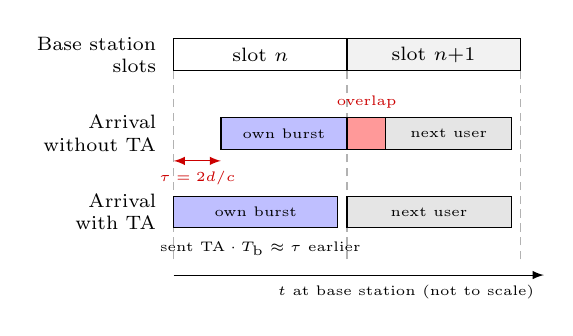
\begin{tikzpicture}[>=latex]
    % Slot width 2.2, burst occupies 148 of 156.25 bit periods, delay tau not to scale
    \def\W{2.2}
    \def\B{2.084}
    \def\delay{0.6}
    \tikzset{rowlabel/.style={anchor=east, font=\scriptsize, align=right}}

    % Slot boundaries at the base station
    \foreach \x in {0, \W, 2*\W} {
        \draw[densely dashed, gray!60] (\x,0) -- (\x,2.8);
    }

    % Base station slot grid
    \node[rowlabel] at (-0.1,2.6) {Base station\\slots};
    \draw[fill=white] (0,2.4) rectangle (\W,2.8);
    \node[font=\scriptsize] at ({\W/2},2.6) {slot $n$};
    \draw[fill=gray!10] (\W,2.4) rectangle (2*\W,2.8);
    \node[font=\scriptsize] at ({1.5*\W},2.6) {slot $n{+}1$};

    % Arrival without timing advance: own burst late by tau, overlaps next user
    \node[rowlabel] at (-0.1,1.6) {Arrival\\without TA};
    \draw[fill=gray!20] (\W,1.4) rectangle ({\W+\B},1.8);
    \node[font=\tiny] at ({\W+\B/2+0.25},1.6) {next user};
    \draw[fill=blue!25] (\delay,1.4) rectangle (\W,1.8);
    \draw[fill=red!40] (\W,1.4) rectangle ({\delay+\B},1.8);
    \node[font=\tiny] at ({(\delay+\W)/2},1.6) {own burst};
    \node[font=\tiny, text=red!80!black] at ({\W+0.25},2.0) {overlap};
    \draw[<->, red!80!black] (0,1.25) -- (\delay,1.25)
        node[midway, below, font=\tiny] {$\tau = 2d/c$};

    % Arrival with timing advance: own burst aligned, guard period separates users
    \node[rowlabel] at (-0.1,0.6) {Arrival\\with TA};
    \draw[fill=blue!25] (0,0.4) rectangle (\B,0.8);
    \node[font=\tiny] at ({\B/2},0.6) {own burst};
    \draw[fill=gray!20] (\W,0.4) rectangle ({\W+\B},0.8);
    \node[font=\tiny] at ({\W+\B/2},0.6) {next user};
    \node[font=\tiny, anchor=north] at ({\W/2},0.35) {sent $\mathrm{TA}\cdot T_\mathrm{b} \approx \tau$ earlier};

    % Time axis
    \draw[->] (0,-0.2) -- ({2*\W+0.3},-0.2)
        node[below left, font=\tiny] {$t$ at base station (not to scale)};
\end{tikzpicture}
